\documentclass[12pt, notitlepage]{article}
% \usepackage[bottom = 5cm, top = 5cm, left = 3cm, right = 3cm]{geometry}
\usepackage[margin = 1in]{geometry}
\usepackage[english]{babel}
\usepackage[utf8]{inputenc}
\usepackage[table]{xcolor}
\usepackage{graphicx, booktabs, tikz, csquotes, subcaption, enumitem, dcolumn, pdfpages, amsmath}
\usepackage[font=normalsize]{caption}%,labelfont=bf

\usepackage{endnotes}
\let\footnote=\endnote

\renewcommand*\rmdefault{ppl}

\usepackage{setspace}
\setstretch{1.5}

\usepackage[]{titlesec}
    \titleformat*{\section}{\large\bf}
    \titleformat*{\subsection}{\normalsize\it}

% Bibliography
% \usepackage[natbibapa]{apacite}
\usepackage[round]{natbib}
% \renewcommand{\bibliographytypesize}{\normalsize}
\setlength{\bibsep}{5pt}

\usepackage[colorlinks = TRUE, allcolors = blue]{hyperref}

\widowpenalty=10000
\clubpenalty=10000

\title{\Large Do TJ policies cause backlash?\\Evidence from street name changes in Spain}
\author{Francisco Villamil\footnote{Juan March Institute--Carlos III University of Madrid} \and Laia Balcells\footnote{Georgetown University}}
\date{\today}

% for word counting --------
% \usepackage[none]{hyphenat}
% \usepackage[nomarkers]{endfloat}
% --------------------------

\usepackage{xr}
\externaldocument{appendix}

\begin{document}

\maketitle

\begin{abstract}
\setstretch{1.2}
Memories of old conflicts shape domestic politics long after these conflicts end. Contemporary debates about the Confederacy in the United States or the Francoist regime in Spain suggest that these are sensitive topics that might increase political polarization, particularly when transitional justice policies are implemented to address grievances and political parties mobilize grudges around these policies. One such policy recently debated in Spain is the removal of public symbols linked to a past civil war and subsequent authoritarian regime (i.e., Francoism). However, the empirical evidence on their impact is still limited. This article attempts to fill this gap by exploring the impact of street's renaming. Using difference-in-differences analyses, we show that the removal of Francoist street names has contributed to an increase of electoral support for a new far-right party, Vox, mostly at the expense of a traditional right-wing conservative party, PP. Results suggest that revisiting the past and trying to redress the victims' grievances can cause a backlash among those ideologically aligned with the perpetrator, and that this can be capitalized by political parties.

\vspace{10pt}
\noindent
% \textbf{Keywords:} transitional justice, voting, conflict memories, Spain

\end{abstract}
\setstretch{1.5}

\newpage
\section*{Introduction}

Memories of contested historical events shape domestic politics across the world. One way in which historical memory is formed and reproduced is through symbols such as statues or street names, and their establishment (or removal) constitutes a policy that is often related to Transitional Justice (TJ) processes in societies coming out from authoritarian or conflicted pasts. These forms of ``symbolic TJ policies'' are considered important to facilitate national reconciliation.

% and the public display of a contentious past related to the Civil War and slavery.
%Removing these symbols, a transitional justice (thereafter, TJ) policy, is defended on the grounds that they represent ideas that are no longer acceptable and constitute a roadblock to reconciliation.

Yet, the policy of symbol removals is not free of controversy. In Ukraine, the removal of Soviet statues during the `Leninopad' has generated backlash among sympathizers of the former authoritarian regime \citep{Rozenas:2021}. In the South of the United States, there have been several instances of right-wing or white supremacist protests when statues of Confederates have been torn down, and there is a heated policy and scholarly debate about whether these statues should remain in public spaces or not \citep{Grossman:2016}.
%In some cases, these protests have turned violent.
%The 2017 `Unite the Right' rally in Charlottesville, Virginia, opposing the removal of a Robert E Lee statue, escalated into violence and resulted in the death of one person when a white supremacist drove his car into a crowd of counter-protesters.

%In Germany, the co-leader of Alternative for Germany (AfD) dubbed the Berlin Holocaust Museum a ``monument of shame'' \citep{Laub:2018aa}. In Poland, the right-wing Law and Justice (PiS) party has recently changed the National Memory Law, ``threatening to prosecute anyone claiming that the Polish Nation was responsible for Nazi crimes'' \citep[][183]{Zubrzycki:2020aa}.

In this article, we ask if TJ symbolic policies cause backlash. If yes, what are the political consequences of such backlash? If individuals feel aggrieved about symbols of a given past regime being removed, this can be used by social movements or political parties to build further support.
In this article, we explore a potential backlash effect of the removal of public symbols linked to the Francoist regime in Spain, where memories of the Civil War (1936--1939) and the subsequent dictatorship are divisive and potentially polarizing \citep{Balcells:2012aa}.
Our design exploits some of the changes brought about in Spain by the 2007 Law of Historical Memory, which introduced a mandate to remove Francoist symbols from public spaces, including street names. We examine whether streets' renaming generated an increase in electoral support for Vox, a relatively new far-right party.
%Thus fringe party represents a hard version of Spanish nationalism. Its discourse glorifies Spain's imperial past and its national unity, and it also condemns peripheral nationalisms and any attempt at redressing the official memory imposed by the Franco regime..}

While traditional conservative parties in Spain have been generally opposed to TJ policies promoted by left-wing governments and have been adamant to stick to the `pact of forgetting' that characterized the transition to democracy in the late 1970s \citep[e.g.][]{Fuente:1980aa}, the far-right was been more resolute in whitewashing the Francoist regime and defending the preservation of its memory.
In response to recent TJ policies, Vox has fiercely tried to capitalize discontentment among Spaniards who do not support such policies.\footnote{Vox is a relatively new party which promotes a discourse based on authoritarian conservatism and a hard-line version of Spanish nationalism. It originated in 2013 from a split in the traditional right-wing party (Partido Popular, or PP). It shares with other populist right-wing parties in Europe a nativist ideology and a rejection of immigration, gender policies, and the social welfare state \citep{Turnbull-Dugarte:2019aa, Turnbull-Dugarte:2020aa}.} For example, they have been vocally opposed to Francoist symbols removed from public spaces, or to the removal of Francisco Franco's remains from the Valley of the Fallen's mausoleum \citep{Taladrid:2019aa}.\footnote{Characterizing the Law of Historical Memory as an instrument of leftist propaganda, Vox campaigned on the national unity of Spain as a way of leaving behind historical divisions and enacted the figure of Francisco Franco as an important political leader who brought peace and stability to the country.} Yet, we do not know whether this strategy has electorally benefited this far-right party or not, and identifying causality is thorny because of counfounding events. For example, in the 2017 secessionist crisis in Catalonia, Vox has been actively involved in the judicial prosecution of secessionist leaders, and has attempted to mount as true guarantor's of Spanish territorial unity.

%We aim to shade some light on this question.
%Originated from a split within the mainstream right-wing party (Partido Popular), Vox represents a hard version of Spanish nationalism.
%Its discourse glorifies Spain's imperial past and its national unity.
%It also condemns peripheral nationalisms and any attempt at redressing the official memory imposed by the Franco regime.
%In this study, we probe whether the removal of Francoist street names accounts for variation in support for Vox.
%Our results support the backlash hypothesis.
%Cross-sectional analyses show there is a correlation between the removal of Francoist street names and electoral support for Vox in Spanish 2019 elections.
%Also, in order to get closer to a causal identification,
In this study, we implement a difference-in-differences (DiD) design where we analyze the impact of Francoist street name removals on the growth of Vox electoral support between June 2016 and April 2019.
%Focusing only on a subset of municipalities that still had Francoist street names in June 2016,
We find that electoral support for Vox increased around 6\% more in municipalities where there was a removal of Francoist street names between June 2016 and April 2019 than in places without such removals. Support for the Partido Popular (PP) decreased 8\% more in those same municipalities, while support for the the socialist party (PSOE) did not vary, suggesting a potential link to increased asymmetric polarization by which there is increased radicalization only in one sector of society (in this case, the right).
%While they cannot directly generalize due to the role of contextual factors, our findings have implications about symbolic TJ and other historical memory polices in other parts of the world.

%The politics of memory and the revision of a country's history are key issues in contemporary politics.
%National traditions and symbols across the world are being criticized because of their racial or ideological overtones.
%Even though those who support these revision policies usually claim that they promote reconciliation, our argument is that can also have the unintended side effect of increasing political polarization.

\section*{The effects of ``symbolic'' TJ policies}

After regime transitions or violent episodes, countries face the need to come to terms with the past \citep{Elster:2004aa}. To this end, countries often rely on different TJ policies, such as trials, truth commissions, reparations, amnesties, or ``symbolic'' measures (i.e., museums, memorials) \citep{De-Brito:2001aa, Elster:2004aa, Balasco:2013aa}. All these diverse measures aim to serve justice, redress grievances, and reduce the probability of conflict recurrence \citep{Loyle:2017aa}. However, the short-term and long-term and consequences of TJ policies are still not clear.

Many scholars praise TJ policies, arguing that they increase the prospect for democracy \citep{Elster:2004aa, Sikkink:2007aa} and reduce the risk of future conflict by increasing accountability for past victimization \citep{Kim:2010aa, Meernik:2010aa}, and redressing grievances \citep{Akhavan:1998aa,  Loyle:2017aa}.

Other authors argue that the positive view on TJ policies is overly optimistic, and that there is scant evidence supporting their beneficial effect \citep{Mendeloff:2004aa, Thoms:2010aa}. Some even claim that TJ policies can have a negative effect on reconciliation and conflict because they can renew social tensions in divided societies \citep{Snyder:2004aa}.
%\footnote{The idea that TJ policies might intensify old hatreds and divisions was precisely one of the arguments held by conservative sectors in Spain against the 2007 Law of Historical Memory.}
%Indeed, the debates about the past related to these TJ policies seem to have played a meaningful role in building a successful electoral discourse among populist right-wing parties in some European countries \citep{Martin:2020aa}.

%Previous research has paid close attention to the formal justice mechanisms of TJ policies, but we know much less about more informal measures of TJ and their effects on public opinion or voting behavior.
%Two recent works constitute a partial exception to this gap.
Trying to shed light on this debate, \cite{Capoccia:2020aa} study the effects of TJ trials on prodemocratic attitudes in West Germany, and find heterogenous effects depending on the type of punishment and the ethnic identity of the defendants. \cite{Balcells:2020aa}, for their part, study the impact of TJ museums with a RCT in Santiago, Chile. They find a single TJ museum visit can have reconciliatory and prodemocracy effects among visitors, and document no evidence of a backlash among those ideologically close to the Pinochet regime.

We contribute to this debate by exploring the effects of a particular subset of TJ policies: the removal of symbols from public spaces. In particular, we focus on the removal of Francoist street names in Spain. Street renaming, just like the removal of statues and other symbols or the building of museums and establishment of historical markers \citep{Ward2021}, are a form of what \citet{Aguilar:2011aa} call ``symbolic Transitional Justice''. Symbolic TJ is very much intertwined with the politics of memory, which involve ``the shaping of collective memory by political actors and institutions'' \citep[][176]{Zubrzycki:2020aa}. While there has been significant research on other aspects of TJ policies such as trials, reparations, or lustration \citep{Nalepa:2010, Loyle:2017aa, voytas:2021}, the study of symbolic TJ is still quite underdeveloped.

In Spain, the Law of Historical Memory (2007), promoted by a left-wing (PSOE) government, constituted an attempt to redress long-held grievances by the victims of the civil war and the Francoist regime. Among other things, it included provisions for the removal of Francoist symbols from public spaces, such as street names and monuments. Some local governments had already changed Francoist street names right after the transition to democracy. Still, these changes depended on an active decision made at the local level. In hundreds of municipalities, either because the historical memory issue was less salient or because local politicians actively rejected the change, many streets were still named after Francoist symbols or leaders.
The 2007 Law prompted local governments to be proactive and offered local associations a legal platform to pressure their local councils to remove these symbols. Anecdotally, we know that these policies generated some backlash among right-wingers, but we do not know if this backlash was systematic, and the extent to which it benefited the far-right, which tried to exploit it electorally. We test this hypothesis with granular data from Spanish municipalities.
%``backlash hypothesis'', namely, that removing public symbols will mobilize and radicalize those who are ideologically closer to these symbols. If this hypothesis is true, in the context of Spain, we would expect that the removal of Francoism symbols would lead to an increase in support for the far-right.

%\section*{Conflict memories and authoritarian backlash in Spain}

%We exploit two recent phenomena in Spanish politics: the consequences of the Law of Historical Memory and the recent rise of a far-right party, Vox.%, whose discourse rests heavily on the version of Spanish nationalism supported by Francoism.

%In Spain, the Law of Historical Memory (2007), promoted by a left-wing (PSOE) government, constituted an attempt to redress long-held grievances by the victims of the civil war and the Francoist regime. Among other things, it included provisions for the removal of Francoist symbols from public spaces, such as street names and monuments.

%Some local governments had already changed Francoist street names right after the transition to democracy.
%For instance, the \textit{Paseo de la Castellana} and the \textit{Avinguda Diagonal}, two of the main arteries of Madrid and Barcelona, respectively, were named \textit{Avenida del Generalísimo Franco} until 1979.
%However, these changes depended on an active decision made at the local level.
%In many places, either because the civil war/Francoist issue was less salient or because local politicians actively rejected the change, many streets were still named after Francoist symbols or leaders.
%The 2007 Law prompted local governments to act and offered local associations a legal platform to pressure their local councils.% to promote street name changes.
%\footenote{In fact, the Law of Historical Memory promoted and funded local `memory associations' that reviewed the local history and organized the exhumation of local mass graves.}

%These policies were hotly contested by particular sectors of Spanish society. By the late 2000s, even if the 2007 Law had a broad support in Spanish society, a significant proportion of the population still disagreed with its provisions \citep{Aguilar:2011aa}.
%Even from the very first years of democratic rule, rightist parties rejected the change of street names or the removal of public monuments by saying that revisiting history only brought old-seated divisions back \citep[e.g.][]{Fuente:1980aa}.
%\footnote{The exhumation of Francisco Franco from the Valley of the Fallen in late 2019 is probably the latest high-key example of the implementation of this law and the political tension it brought about \citep{Taladrid:2019aa}.}
%

%To analyze the effect of TJ policies aimed at removing symbols, we focus on electoral support for Vox as our measure for far-right ideological preferences.
%Vox is a relatively new party which promotes a discourse based on authoritarian conservatism and a hard-line version of Spanish nationalism. It originated in 2013 from a split in the traditional right-wing party (Partido Popular, or PP). It shares with other populist right-wing parties in Europe a nativist ideology and a rejection of immigration, gender policies, and the social welfare state \citep{Turnbull-Dugarte:2019aa, Turnbull-Dugarte:2020aa}.
%This discourse mirrors the `forgetting` policy developed by Franco in the postwar period \citep{Palomares:2004aa}.


%We make use of these two events to assess whether the politics of memory in Spain caused a backlash towards positions closer to the ideology of the Francoist regime. In particular, we measure whether the renaming of streets led to increased  support for Vox.
%Our expectation is that the relationship will be positive, supporting the backlash hypothesis.

\section*{Empirics}

We implement a DiD design analyzing the effect of Francoist street name removals on the growth of local electoral support for Vox between June 2016 and April 2019 elections.
We focus on this time period for two reasons.
First, given that Vox first participated in national elections in December 2015, the 2016--2019 period is the only electoral period longer than six months in which it is possible to see changes in support for Vox.
And second, it was precisely during this period when Vox experienced a growth in support that let the party become one of the key electoral players in Spain.

Limiting the sample to all municipalities that still had at least one street with a Francoist name in June 2016, our main models aim to identify whether Vox grew more in municipalities that removed Francoist street names. % We discuss each of the variables below.

\subsection*{Francoist street name removal}

To build our main independent variable, we use data from the  Spanish National Statistical Institute \citep{INE:2020aa} identifying all the streets in Spain at different points in time. The INE offers data on all existing streets on June 30th and December 31st every year since late 2010.\footnote{The INE also offers one-time data for June 2001.}
Using the official ID number for each street, we track name changes over time.

We then identify streets names after Francoist symbols or figures.
We use the list published by the Madrid City Council in 2017, following a report by a specially designated commission,\footnote{The full list is available online at https://bit.ly/37cLGgk (accessed 26/11/2020).} and manually expanded it by selecting Francoist names among the most frequent changes (e.g., `Jos\'e Antonio', `Calvo Sotelo', `Generalísimo', `General Franco').
We show the full list in the Appendix (section~\ref{app:franc_names_list}).
Our main variable is a binary indicator of Francoist street name removal between June 30th, 2016 and December 31st, 2019.\footnote{See section~\ref{app:treatment_strength} in the appendix for more details about the binary coding.}

Figure~\ref{fig:changes_time} shows the number of Francoist street name removals during every six-month period since 2011. There is a spike after 2016, precisely the period we study. The main reason behind this increase is that, at the local level, the different legal battles or lobbying campaigns to remove Francoist names took time.
In mid-2016, Olmedo, Valladolid, was the first municipality to be sentenced for not complying with the 2007 LHM \citep{El-Norte-de-Castilla:2016aa}.
Around the same time, many municipalities began facing trials after being sued by local historical memory associations.
Moreover, after 2015, there was an increased institutional activity in favor of street renaming, partly as a result of the PP losing grip of a number of municipal and regional governments in the 2015 elections \citep[e.g.][]{Vazquez:2016aa, El-Comercio:2016ab}.
%, such as Llanes, Asturias \citep{El-Comercio:2016aa}.
%Second, the decrease in votes for the mainstream right-wing party in the 2015 local and regional elections changed the balance of power which, together with a general increase in the salience of this issue, meant more institutional activity in this direction

\begin{figure*}[htb!]
\centering

  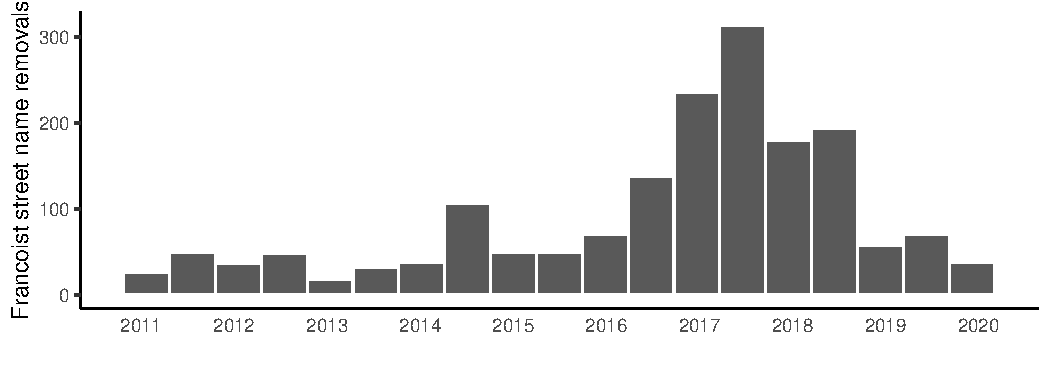
\includegraphics[width = 0.8\textwidth]{img/changes_by_year}

  \caption{Number of Francoist street name removals over time (2011-2020)}\label{fig:changes_time}

  \vspace{5pt}

  % \parbox[t]{0.84\textwidth}{\footnotesize{\textbf{Note:} Data from INE. After 2011, data was published every 6 months. Before that date, there is only one data point, in June 2001.}}

\end{figure*}

The post-2016 increase could bias the results if it was related to political dynamics that also explain the change in political preferences.
However, the data suggests this is not the case.
We discuss this issue more in depth below and in the Appendix (section~\ref{app:treated_vs_control_vs_outsample}).
%We discuss at length the differences between municipalities in and out of the sample in the appendix (section~\ref{app:treated_vs_control_vs_outsample}).% we show that most of the municipalities that removed Francoist street names were small municipalities that had more Francoist street names to start with, and mostly in provinces in the central regions of Spain, which is in line with the factors discussed above.

\subsection*{Vox electoral support}

We exploit support for Vox as our main dependent variable.%, using it as a proxy for an authoritarian backlash in political preferences.
We obtained the data from the Spanish Ministry of Interior,\footnote{Results are available at \href{http://www.infoelectoral.mir.es/}{http://www.infoelectoral.mir.es/} (accessed 03/12/2020).}
and calculated the share of valid votes for Vox in each municipality.

In addition, we also use as dependent variables the electoral share for the two mainstream parties, the right-wing Popular Party (\textit{Partido Popular}, PP) and the Spanish Socialist Workers' Party (\textit{Partido Socialista Obrero Español}, PSOE), in order to capture the local shift in political preferences.
%Specifically, given that we are interested in a potential authoritarian backlash among conservative individuals, we want to explore whether the removal of Francoist street names is related to a general shift to the right or an increase in political polarization.

\subsection*{Control variables}

We include a series of control variables at the local level that can be related to the increase in electoral support for Vox.
In particular, we include turnout in April 2019 elections, (logged) population in the 2011 census, the (logged) number of Francoist street names in June 2016, the unemployment rate in January 2016, and a binary indicator of whether a leftist mayor was elected in the May 2015 local elections.
In addition, we also include fixed effects at the region level (Autonomous Communities).
We show summary statistics in the Appendix (section~\ref{app:descriptives}).

\subsection*{Models}

We run OLS regression on the electoral support for Vox, PP, and PSOE in June 2016 and April 2019 elections as the dependent variable, and an indicator of street name removal between June 2016 and December 2018 as our main independent variable.
The model is defined as

\begin{equation}
\begin{split}
    Share_{it} =&  \beta_0 + \beta_1 Removal_{it} + \beta_2 April2019_{it} +\\
    &\beta_3 (Removal_{it} \times April2019_{it}) + \beta^\top \mathbf{x}_{it} + \alpha_{it} + \epsilon_{it}
\end{split}
\end{equation}

Where $\mathbf{x}_{it}$ is a vector of covariates, $\alpha_{it}$ are region fixed effects, and $\epsilon_{it}$ is the error term.
The effect of street name removals is captured by $\beta_3$, the interaction between the $t_{1}$ (April 2019) and treatment (name removal) variables.

As explained above, we only include in the sample municipalities that still had Francoist street names in June 2016.
Table~\ref{tab:sample_trt} classifies the municipalities in the sample, and how many of them are in the control and treatment conditions.
In addition, in order to use the same sample across the models for each party, we exclude from the sample municipalities where Vox did not participate in June 2016 elections, which leaves us with a total of 1169 municipalities.
We include detailed information about these groups in the Appendix (sections~\ref{app:descriptives}-\ref{app:treated_vs_control_vs_outsample}), as well as models for PP and PSOE using the full sample (section~\ref{app:robustness_did}).

\begin{table}[!htbp] \centering
\caption{DiD sample classification}
\label{tab:sample_trt}
\small
\begin{tabular}{lcc}
\\[-1.8ex]\hline
\hline \\[-1.8ex]
\multicolumn{1}{p{3cm}}{\hspace{3cm} Francoist names} & \multicolumn{2}{p{3.5cm}}{Removed Francoist names, 2016--2018?}\\
in June 2016? & No & Yes \\
\cline{2-3} \\[-1.8ex]
No & 6455 & 0 \\
 & (100\%) & (0\%) \\
Yes (DiD sample) \hspace{2cm} & 1184 & 454 \\
 & (72\%) & (28\%) \\
\\[-1.8ex]\hline
\hline \\[-1.8ex]
\multicolumn{3}{c}{\parbox[t]{0.55\textwidth}{\textit{Note:} Row percentages. Changes in 2016--2018 refer to the period between 01/07/2016 and 31/12/2018.}}\\
\end{tabular}
\end{table}


Limiting the sample implies that the the control group---those municipalities that did not change street names during this period---is probably more rightist than the average (compared to municipalities out of the sample), as more leftist municipalities are more likely to have already changed Francoist street names before 2016.
Indeed, some municipalities that still had not changed Francoist names by late 2018 were portrayed as the `resistance' to the Law of Historical Memory \citep{Blanco-Elipe:2018aa}, as they actively avoided doing so.
This dodging of the Law was possible either because of delays in the legal procedures or some form of `foot-dragging' by local authorities.
Because of this, the selection bias should go against our hypothesis, in the sense that the control group is comprised by municipalities where Vox is likely to have grown more between 2016 and 2019.
We provide further empirical evidence on this in the Appendix (section~\ref{app:treated_vs_control_vs_outsample}), including a test of the parallel trends assumption (section~\ref{app:robustness_did}).

\section*{Results}

Table~\ref{tab:did_deco} shows the mean electoral share for each of the three parties in 2016 and 2019 elections, for the treated and control groups.
We also show the base difference in differences.

\begin{table}[!htbp] \centering
\caption{Mean electoral share in sample}
\label{tab:did_deco}
\small
\begin{tabular}{lccccccc}
\\[-1.8ex]\hline
\hline \\[-1.8ex]
\\[-1.8ex]
& \multicolumn{3}{c}{June 2016} & \multicolumn{3}{c}{April 2019} & \\\\[-1.8ex]
\cline{2-7}\\[-1.8ex]
Party & $Control$ & $Treated$ & $\Delta$ & $Control$ & $Treated$ & $\Delta$ & $\Delta_{2019} - \Delta_{2016}$ \\
\hline \\[-1.8ex]
Vox & 0.21 & 0.21 & 0 & 12.54 & 13.28 & 0.74 & 0.74 \\
PP & 41.22 & 46.77 & 5.55 & 23.83 & 27.68 & 3.85 & -1.7 \\
PSOE & 29.13 & 28.01 & -1.12 & 33.38 & 32.03 & -1.35 & -0.23 \\
\hline
\hline \\[-1.8ex]
\end{tabular}
\end{table}



Table~\ref{tab:main_did} shows the results of the DiD analyses.
In order to see the results more clearly, figure~\ref{fig:main_did} shows the simulated DiD estimate of the Francoist street name removal, using the models with control variables.


% Table created by stargazer v.5.2.2 by Marek Hlavac, Harvard University. E-mail: hlavac at fas.harvard.edu
% Date and time: Thu, May 27, 2021 - 17:29:25
% Requires LaTeX packages: dcolumn 
\begin{table}[!htbp] \centering 
  \caption{Francoist street name removal and increase in electoral support for parties} 
  \label{tab:main_did} 
\small 
\begin{tabular}{@{\extracolsep{-20pt}}lD{.}{.}{-3} D{.}{.}{-3} D{.}{.}{-3} } 
\\[-1.8ex]\hline 
\hline \\[-1.8ex] 
\\[-1.8ex] & \multicolumn{1}{c}{VOX} & \multicolumn{1}{c}{PP} & \multicolumn{1}{c}{PSOE} \\ 
\\[-1.8ex] & \multicolumn{1}{c}{(1)} & \multicolumn{1}{c}{(2)} & \multicolumn{1}{c}{(3)}\\ 
\hline \\[-1.8ex] 
 (Intercept) & -1.470^{**} & 56.375^{***} & 34.870^{***} \\ 
  & (0.451) & (0.922) & (0.876) \\ 
  Francoist street name removal & -0.132 & 1.158^{*} & -0.159 \\ 
  & (0.262) & (0.476) & (0.453) \\ 
  Election April 2019 & 12.319^{***} & -17.406^{***} & 4.629^{***} \\ 
  & (0.167) & (0.338) & (0.320) \\ 
  Francoist removal $\times$ April 2019 & 0.724^{*} & -1.405^{*} & -0.434 \\ 
  & (0.352) & (0.639) & (0.607) \\ 
 \hline \\[-1.8ex] 
Controls & \multicolumn{1}{c}{Yes} & \multicolumn{1}{c}{Yes} & \multicolumn{1}{c}{Yes} \\ 
CCAA Fixed Effects & \multicolumn{1}{c}{Yes} & \multicolumn{1}{c}{Yes} & \multicolumn{1}{c}{Yes} \\ 
Observations & \multicolumn{1}{c}{2,310} & \multicolumn{1}{c}{3,223} & \multicolumn{1}{c}{3,242} \\ 
R$^{2}$ & \multicolumn{1}{c}{0.768} & \multicolumn{1}{c}{0.720} & \multicolumn{1}{c}{0.482} \\ 
Adjusted R$^{2}$ & \multicolumn{1}{c}{0.766} & \multicolumn{1}{c}{0.717} & \multicolumn{1}{c}{0.478} \\ 
\hline 
\hline \\[-1.8ex] 
\multicolumn{4}{c}{\parbox[t]{0.75\textwidth}{\textit{Note:} $+ p<0.1; * p<0.05; ** p<0.01; *** p<0.001$. Only municipalities that had at least one street with a Francoist name in $t_{0}$ were included in the sample.}} \\ 
\end{tabular} 
\end{table} 


\begin{figure*}[htb!]
\centering

  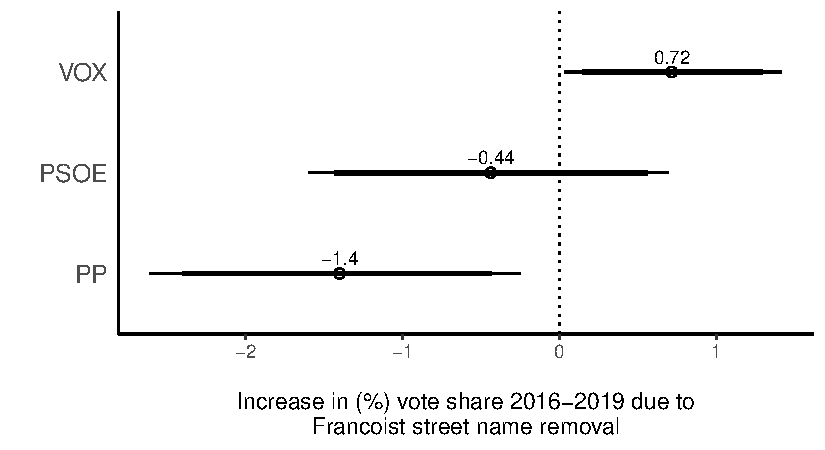
\includegraphics[width = 0.6\textwidth]{img/DiD_estimates}

  \caption{DiD estimates of Francoist street name removal on vote change, obtained from simulations (mean and 90\%/95\% CIs)}\label{fig:main_did}

\end{figure*}

Results support the idea that the changes caused a backlash.
On the one hand, in municipalities where Francoist street names were removed, Vox increased its support 0.7 points more.
Considering that the nation-wide electoral share of Vox in April 2019 was 10.3\%, this effect is significant: the change in electoral support was around 6\% higher in these municipalities.
On the other hand, the removal of Francoist street names is related to an even higher decrease in electoral support for PP, of almost 1.5 points.
However, it did not have any significant effect on electoral support for PSOE, which suggests the change in political preferences took place among rightist individuals.
This last result is coherent with the idea that there changes were linked not only to the name removals but to mobilization strategies of the far-right.

The results could be confounded if the removal of Francoist street names was explained by the same factors that also explain a shift to far-right preferences.
One possibility is that these street name changes, which took place relatively late, took place in more conservative areas where Spanish nationalism was stronger.
%We believe that any selection bias in the sample should be in the opposite direction from the results.
In this case, we should see different trends before 2016 between municipalities that later had a change and those that did not.
Figure~\ref{fig:par_trends_norm} shows normalized electoral trends among control and treated groups for PP and Vox.
Even though in the case of Vox we can only go as far back as December 2015 elections, there are no differing trends before 2016 for the two parties for which we find an effect.
In the Appendix, we also include more detailed models analyzing the parallel trends assumption for Vox, PP, and PSOE (section~\ref{app:robustness_did}).

\begin{figure*}[htb!]
\centering

  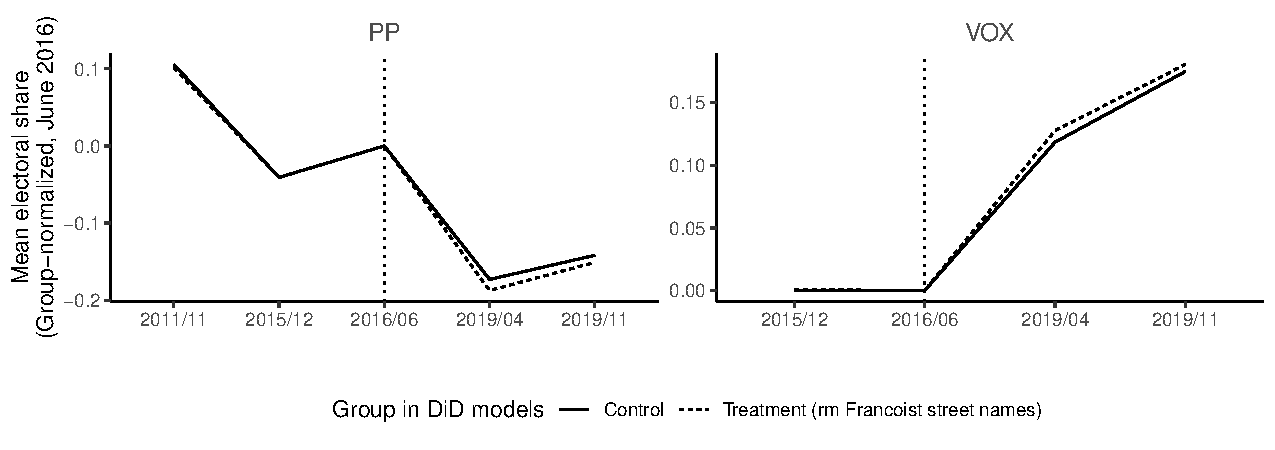
\includegraphics[width = \textwidth]{img/par_trends_norm}

  \caption{Pre- and post-treatment trends in Vox and PP electoral share}\label{fig:par_trends_norm}

\end{figure*}


We also include a number of additional analyses in the Appendix.
On the one hand, we show cross-sectional models (section~\ref{app:crosssec}) using the independent variable in continuous form, tracking Francoist street name removals during different periods (including changes between 2001 and 2019), and using as the dependent variable support for Vox in November 2019 elections as well as the change in support between April and November 2019.
Results are coherent with the DiD analyses, and show that Francoist street name removals account for the growth in support between 2016 and 2019 but not for the changes between April and November 2019, which suggests that any local effect due to a backlash over the politics of memory took place prior to April 2019.

On the other hand, we also test the robustness of the DiD analyses to a different specifications (section~\ref{app:robustness_did}), namely, including the main independent variable in continuous form (logged number of street name removals), restricting the sample to municipalities where Vox had more than 0 votes in 2016, and changing the independent variable so it also registers changes that were registered in the first half of 2019.
We also show results from first-difference models (section~\ref{app:first_diff}).
In every case, results do not change significantly when using alternative specifications and support the main findings.

\section*{Conclusion}

In this article, we have explored the political effect of the removal of Francoist street names in Spain.
Our results suggest that this policy can cause a backlash. Using local-level data, we find a short-term positive effect of these changes on the increase in support for the far-right party, Vox, which has recently gained steam with a discourse grounded in an authoritarian and exclusionary version of Spanish nationalism.

The results from our analyses echo recent debates about symbolic TJ policies and memories of past conflicts in other countries. For example, the debate in the United States over the Confederate symbols shows that this type of policies can generate political instability and even spark political violence. In Ukraine, the removal of Soviet monuments has also generated controverly and likely benefited pro-soviet political parties \citep{Rozenas:2021}. Our goal is not to take a normative stand against these policies. We believe that, in spite of these short term backlash effects, they can be highly beneficial in the long run (these measures could well contribute to national reconciliation down the road). Moreover, we  show that TJ symbolic policies might cause a backlash and have political consequences, as it has been the case of Ukraine or Spain, where some political parties have taken electoral advantage of it. Yet, this backlash should not be not an automatic outcome of these policies and can perhaps be palliated by actions of other political parties. For example, countering narratives or compensating the aggrieved in other ways (i.e., relocating these symbols into a museum) could limit the extent to which extremist or populist parties capitalize their discontentment. The extent to which such remedial policies can work is nonetheless out of the scope of this paper. Finally, while we have found evidence regarding the removal of symbols, other TJ policies might not have to similar backlash effects. For instance, recent research shows that TJ museums can have a positive effect on reconciliation \citep{Balcells:2020aa}, and that reparations can political engagement among victims \citep{voytas:2021}. The overall effect of TJ might depend on the balance between different measures \citep{Olsen:2010aa, Loyle:2017aa}.
Overall, this article contributes to the scholarly debate on the effectiveness of TJ policies, a debate that remains open and will require further research.

%Far from arguing against these types of policies, we think it is important to be aware of these potentially undesired effects when designing transitional justice policies. Specifically, two aspects merit further attention:
 %Moreover, even if it is the case that the removal of public symbols might cause backlash, this might not be the case for

%All in all, this article focuses on a relatively unexplored question. Exploiting recent political events in Spain, we offer empirical evidence suggesting that, in the short run, symbolic transitional justice policies might have an unintended effect: an increased support for political actors siding with the former regime or perpetrators of violence.


\newpage
\begingroup
\parindent 0pt
\parskip 2ex
\def\enotesize{\normalsize}
\theendnotes
\endgroup

\clearpage
\bibliographystyle{rap}
\bibliography{REF}

\newpage
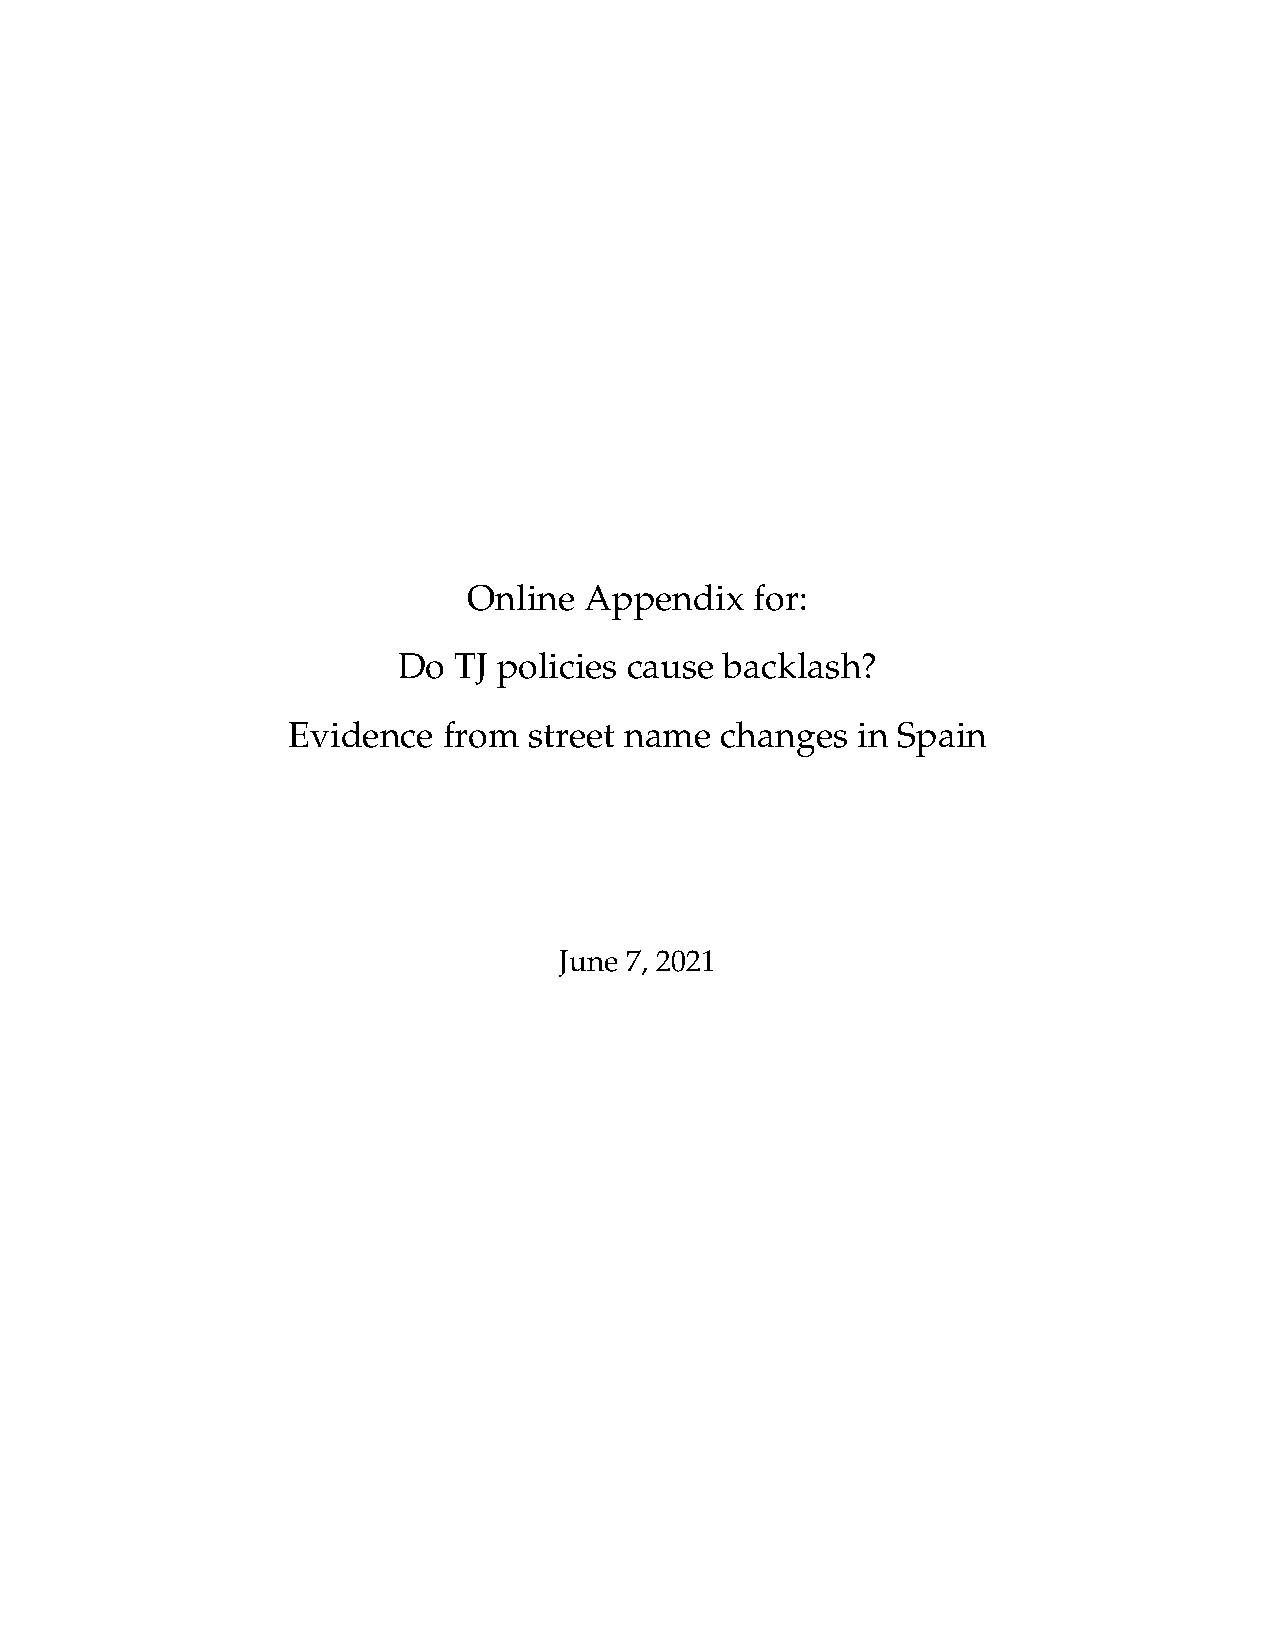
\includepdf[pages=-]{appendix.pdf}

\end{document}
